\documentclass[a4paper,11pt]{ctexart}
\usepackage[margin=2.5cm]{geometry}
\usepackage{booktabs}
\usepackage{array}
\usepackage{longtable}
\usepackage{tikz}
\usetikzlibrary{positioning}
\usepackage{hyperref}
\usepackage{enumitem}
\usepackage{fancyhdr}
\usepackage{setspace}

\setcounter{secnumdepth}{4}
\setlength{\parindent}{2em}
\onehalfspacing

\pagestyle{fancy}
\fancyhf{}
\fancyhead[C]{\small DL/T 790.6---2010/IEC 61334-6:2000}
\fancyfoot[C]{\thepage}

\begin{document}

%========== 封面信息 ==========
\begin{center}
\vspace*{2cm}

{\Large ICS 27.100 \qquad F21}

\vspace{1cm}
备案号：29043---2010

\vspace{2cm}
{\LARGE\bfseries 中华人民共和国电力行业标准}

\vspace{1cm}
{\Large DL/T 790.6---2010 / IEC 61334-6:2000}

\vspace{1.5cm}
{\LARGE\bfseries 采用配电线载波的配电自动化\\[0.5em] 第6部分：A-XDR编码规则}

\vspace{1cm}
{\normalsize Distribution automation using distribution line carrier system---\\
Part 6: A-XDR encoding rule}

\vspace{2cm}
2010---05---24发布 \qquad (IEC 61334-6:2000, IDT)\\[0.5em]
2010---10---01实施

\vspace{2cm}
{\Large 国家能源局\ 发布}

\end{center}
\newpage

%========== 前言 ==========
\section*{前言}
\addcontentsline{toc}{section}{前言}

随着我国电网技术的发展，对配电自动化的要求已日益迫切。与传输配电自动化信息的其他通信方式相比，配电线载波可以降低建设投资和运行费用，便于管理，是一种经济实用的通信方式。配电电压不高，但电网结构复杂，信号传输衰减大。针对配电网信号传输特点，自1995年起，国际电工委员会陆续发布了IEC 61334系列的国际标准或技术报告。采用这些文件使之成为我国的标准文件对于我国这方面工作的开展有很好的指导意义，便于与国际接轨。

系列标准DL\,790《采用配电线载波的配电自动化》采用国际系列标准IEC 61334《采用配电线载波的配电自动化》，包括标准和标准化指导性技术文件，共有以下20部分：

\begin{enumerate}[label=\arabic*),leftmargin=2em,itemsep=0.2em]
\item DL/Z 790.11 采用配电线载波的配电自动化 第1部分：总则 第1篇：配电自动化系统的体系结构
\item DL/Z 790.12 采用配电线载波的配电自动化 第1部分：总则 第2篇：制定规范的导则
\item DL/Z 790.14 采用配电线载波的配电自动化 第1-4部分：总则 中低压配电线载波传输参数
\item DL/T 790.31 采用配电线载波的配电自动化 第3部分：配电线载波信号传输要求 第1篇：频带和输出电平
\item DL/T 790.321 采用配电线载波的配电自动化 第3-21部分：配电线载波信号传输要求 中压绝缘电容型相相结合设备
\item DL/T 790.322 采用配电线载波的配电自动化 第3-22部分：配电线载波信号传输要求 中压相地和注入式屏蔽地结合设备
\item DL/T 790.41 采用配电线载波的配电自动化 第4部分：数据通信协议 第1篇：通信系统参考模型
\item DL/T 790.432 采用配电线载波的配电自动化 第4-32部分：数据通信协议 数据链路层---逻辑链路控制
\item DL/T 790.433 采用配电线载波的配电自动化 第4-33部分：数据通信协议 数据链路层---面向连接的协议
\item DL/T 790.441 采用配电线载波的配电自动化 第4-41部分：数据通信协议 应用层协议---配电线报文规范
\item DL/T 790.442 采用配电线载波的配电自动化 第4-42部分：数据通信协议 应用协议 应用层
\item DL/T 790.4511 采用配电线载波的配电自动化 第4-511部分：数据通信协议 系统管理 CIASE协议
\item DL/T 790.4512 采用配电线载波的配电自动化 第4-512部分：数据通信协议 系统管理 采用协议集的系统管理信息库
\item DL/T 790.461 采用配电线载波的配电自动化 第4-61部分：数据通信协议 网络层 无连接协议
\item DL/T 790.51 采用配电线载波的配电自动化 第5部分：低层协议集 第1篇：扩频型移频键控(S-FSK)协议
\item DL/Z 790.52 采用配电线载波的配电自动化 第5-2部分：低层协议集 移频键控(FSK)协议
\item DL/Z 790.53 采用配电线载波的配电自动化 第5-3部分：低层协议集 自适应宽带扩频(SS-AW)协议
\item DL/Z 790.54 采用配电线载波的配电自动化 第5-4部分：低层协议集 多载波调制(MCM)协议
\item DL/Z 790.55 采用配电线载波的配电自动化 第5-5部分：低层协议集 快速跳频扩频通信(SS-FFH)协议
\item DL/T 790.6 采用配电线载波的配电自动化 第6部分：A-XDR编码规则
\end{enumerate}

本部分等同采用IEC 61334-6:2000《采用配电线载波的配电自动化 第6部分：A-XDR编码规则》（英文版）。

本部分的附录A、附录B、附录C为资料性附录。

本部分由中国电力企业联合会提出。

本部分由全国电力系统管理及其信息交换标准化技术委员会归口。

起草单位：国网电力科学研究院、北京四方继保自动化股份有限公司、中国电力科学研究院。

主要起草人：于跃海、任雁铭、但富中、陈道元、沐连顺。

在执行过程中的意见或建议反馈至中国电力企业联合会标准化中心（北京市白广路二条1号，100761）。

\newpage

%========== 引言 ==========
\section*{引言}
\addcontentsline{toc}{section}{引言}

本部分根据《国家发展改革委办公厅关于印发2007年行业标准修订、制定计划的通知》（发改办工业[2007]1415号）的安排制定。

国际电信联盟（ITU-T）的X.208建议定义了一种形式语言---ASN.1（Abstract Syntax Notation One，抽象语法记法1），使应用层规范能定义需要交换的信息类型\footnote{ASN.1为已定义类型值的规范规定了记法。}。将一组编码规则应用于ASN.1定义的类型的数值可以形成这种信息的一种表示方法。这些编码规则的应用产生了这些数值的转化语法。

虽然人们已经设想了多种编码规则，但是长期以来只有一种BER（Basic Encoding Rule，基本编码规则）用作标准（见ITU-T的X.209）。这主要是因为BER能够满足绝大多数应用的需要。但在某些情况下，它显得冗余。如何采用其他编码规则以避免冗余，是最近开发的一些转化语法标准（DER、CER、PER）的研究目的。这些转化语法标准和BER不同，比BER更适合于某些场合。它们不是通用的，而是专用的。

与通用编码规则不同，DL\,790的本部分定义了一种新的、专用的编码规则---A-XDR，它最适用于DLMS（Distribution Line Message Specification，配电线报文规范，见DL/T 790.441）环境。主要目的是将DLMS的PDU（Protocol Data Unit，协议数据单元）的编码优化\footnote{如只考虑PDU的大小，PER比A-XDR性能好。但是，PER的主要目标是压缩容量，这是通过大量使用位域而不是字节域对不同数值进行编码而获得的。为了进一步减少PDU的大小，它使用了更复杂的PER变量（不对齐的PER），也对类型及数值加以限制。因此，它的压缩是以增加计算负担为代价而获得的。此外，PER有对齐和不对齐两种情况，实现时都必须支持。PER的复杂性使它在DLMS环境下不是优选的。"轻型"的A-XDR编码规则更适合于DLMS环境，这种环境的资源量有时很少。}，包括PDU的字节数量及编码解码的复杂性、所需的编码长度、处理性能和时间等。这个目的通过以下两个基本原则实现：

\begin{enumerate}[label=\alph*)]
\item A-XDR只为ASN.1类型应用于DLMS特殊环境的子集规定编码规则（因此，A-XDR是专用的）；
\item A-XDR规定的是面向字节的编码规则。
\end{enumerate}

\newpage

%========== 目录 ==========
\tableofcontents
\newpage

%========== 第1章 ==========
\section{范围}

本部分定义了A-XDR编码规则，它可用来导出在DLMS核心标准中用ASN.1（见DL/T 790.441--2004）定义的数值类型的转化语法规范。这些A-XDR编码规则也可用于对转化语法解码以识别转化的数据值。

A-XDR编码规则：
\begin{enumerate}[label=\alph*)]
\item 在通信中使用；
\item 是DLMS PDU的优化编码方法。
\end{enumerate}

\noindent\textbf{注}：如A-XDR确是DLMS PDU的优化方法，它将成为基于DLMS的通信协议的默认编码规则。然而，不管是默认的还是可选择的编码规则，作为应用层环境的一部分，它都会在已有协议（如DL/T 790.442）的应用层文件中定义。

%========== 第2章 ==========
\section{规范性引用文件}

下列文件中的条款通过本部分的引用而成为本部分的条款。凡是注日期的引用文件，其随后所有的修改单（不包括勘误的内容）或修订版均不适用于本部分，然而，鼓励根据本部分达成协议的各方研究是否可使用这些文件的最新版本。凡是不注日期的引用文件，其最新版本适用于本部分。

\begin{itemize}[leftmargin=2em]
\item DL/T 790.441--2004 采用配电线载波的配电自动化 第4-41部分：数据通信协议 应用层协议---配电线报文规范（idt IEC 61334-41:1996）
\item DL/T 790.442 采用配电线载波的配电自动化 第4-42部分：数据通信协议 应用协议 应用层（idt IEC 61334-42:1996）
\item ISO/IEC 8825-2:-- 信息技术 ASN.1编码规则 包式编码规则（PER）规范
\item ITU-T X.208:1988 抽象语法记法1（ASN.1）规范
\item ITU-T X.209:-- 基本编码规则
\end{itemize}

%========== 第3章 ==========
\section{A-XDR的一般特征}

本部分规定了一种编码规则，可用于对定义为单一ASN.1类型（最外层的类型）的抽象语法数值进行编码或解码。这种单一ASN.1类型可以是简单类型，也可以是复合类型。复合类型的数据项可以是简单类型或复合类型。

规则利用了DLMS PDU发送端和接收端都用相同的抽象语法规范运行这一事实。

用BER时，抽象语法的任何值的编码结构都是TLV（Type-Length-Value，类型---长度---数值）形式。A-XDR只在必要时才对值的类型和长度编码。如果不知道值的类型，就无法确定编码的结构。这种编码方式使A-XDR不可扩展（见附录A）。

为使A-XDR尽量简单，进行抽象语法编码时，应用以下限制条件。

A-XDR是一种改进的XDR。这种XDR由Unix环境下事实上标准的XDR（eXternal Data Representation，外部数据表示，RFC 1014）发展而来。

\begin{enumerate}[label=\alph*)]
\item 不支持DLMS以外的ASN.1类型数据的编码\footnote{附录B枚举了DLMS规范中使用的ASN.1类型和关键字。}；
\item ASN.1选择（CHOICE）类型数据只用于有显式标记\footnote{A-XDR中的术语"显式标记（explicit tagging）"和"隐式标记（implicit tagging）"在ASN.1和BER中的含义有些不同。在6.7里将解释这些名词，并介绍一个新术语"ASN.1显式标记"。}的数据项。
\end{enumerate}

A-XDR是面向字节的编码规则。这意味着每一部分乃至全部的编码的字节数是整数。

%========== 第4章 ==========
\section{编码结构}

BER编码（见ITU-T的X.209）的基本结构：类型、长度和内容，这三部分在BER中可表示为标识符I（Identifier）、长度L（Length）和内容C（Contents），如图\ref{fig:ber}所示。标识符部分用于标识类型，长度部分用于查找内容区\footnote{实际上，在BER中，长度区并不总表示内容区的长度。BER规定有2种形式的长度域：确定型和不确定型。用确定型时，长度域表示内容域的字节数，而用不确定型则表示内容域以内容结束字节结束。}的末端，内容部分用于传送这种类型的可能值。

\begin{figure}[htbp]
\centering
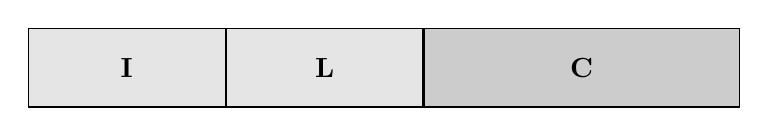
\begin{tikzpicture}
\node[draw, minimum width=2.5cm, minimum height=1cm, fill=gray!20] (I) {\textbf{I}};
\node[draw, minimum width=2.5cm, minimum height=1cm, fill=gray!20, right=0pt of I] (L) {\textbf{L}};
\node[draw, minimum width=4cm, minimum height=1cm, fill=gray!40, right=0pt of L] (C) {\textbf{C}};
\end{tikzpicture}
\caption{BER编码的基本结构}\label{fig:ber}
\end{figure}

内容域可简化为一系列字节\footnote{零个或多个。}（原始编码）或一系列嵌套编码（构造编码），如图\ref{fig:ber-constructed}所示。

\begin{figure}[htbp]
\centering
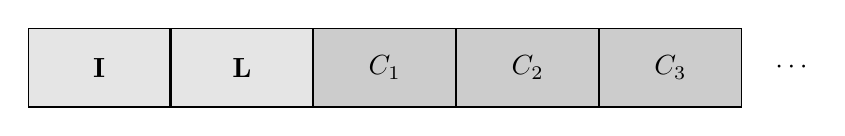
\begin{tikzpicture}
\node[draw, minimum width=1.8cm, minimum height=1cm, fill=gray!20] (I) {\textbf{I}};
\node[draw, minimum width=1.8cm, minimum height=1cm, fill=gray!20, right=0pt of I] (L) {\textbf{L}};
\node[draw, minimum width=1.8cm, minimum height=1cm, fill=gray!40, right=0pt of L] (C1) {$C_1$};
\node[draw, minimum width=1.8cm, minimum height=1cm, fill=gray!40, right=0pt of C1] (C2) {$C_2$};
\node[draw, minimum width=1.8cm, minimum height=1cm, fill=gray!40, right=0pt of C2] (C3) {$C_3$};
\node[right=0.3cm of C3] {$\cdots$};
\end{tikzpicture}
\caption{构造BER的编码结构}\label{fig:ber-constructed}
\end{figure}

嵌套的深度按需要决定，并以原始编码或空内容的构造编码结束。

A-XDR的编码结构与BER基本相同，但为了利用DLMS PDU发送端和接收端按同样的抽象语法规范运行这一事实，当标识符和长度域传送冗余的信息时，A-XDR就不对它们编码（不对其中一个域或两个域编码不会导致编码不可解释或含糊不清）。因此，A-XDR编码的结构如图\ref{fig:axdr}所示。

\begin{figure}[htbp]
\centering
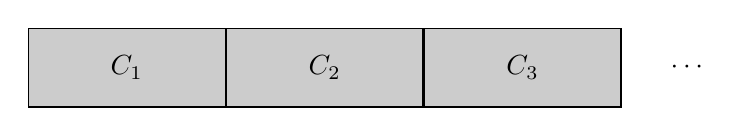
\begin{tikzpicture}
\node[draw, minimum width=2.5cm, minimum height=1cm, fill=gray!40] (C1) {$C_1$};
\node[draw, minimum width=2.5cm, minimum height=1cm, fill=gray!40, right=0pt of C1] (C2) {$C_2$};
\node[draw, minimum width=2.5cm, minimum height=1cm, fill=gray!40, right=0pt of C2] (C3) {$C_3$};
\node[right=0.5cm of C3] {$\cdots$};
\end{tikzpicture}
\caption{构造A-XDR编码的结构}\label{fig:axdr}
\end{figure}

A-XDR编码规则规定：
\begin{itemize}
\item 用于内容域的编码规则；
\item 如有长度域，对长度域编码；
\item 如有标识域，对标识域编码。
\end{itemize}

以下面ASN.1复合类型为例：
\begin{verbatim}
Value ::= SEQUENCE {
    A  Integer16,
    B  Unsigned16
}
\end{verbatim}

\noindent 其中：
\begin{verbatim}
Integer16  ::= INTEGER(-32768..32767)
Unsigned16 ::= INTEGER(0..65535)
\end{verbatim}

\noindent 假设对A和B编码，其值分别为0x1234和0x5678。

上述序列的BER编码如下\footnote{A-XDR只在特殊情况下需要标识（例如：当本例的SEQUENCE是CHOICE类型的选择中的一个时）。}：

\begin{center}
\texttt{30~~06~~02~~02~~12~~34~~02~~02~~56~~78}
\end{center}

\noindent 其中\texttt{30}为序列标识，\texttt{06}为长度，\texttt{02}为A的标识，\texttt{02}为A的长度，\texttt{12~~34}为A的数值，\texttt{02}为B的标识，\texttt{02}为B的长度，\texttt{56~~78}为B的数值。

同一序列的A-XDR编码如下：

\begin{center}
\texttt{12~~34~~56~~78}
\end{center}

%========== 第5章 ==========
\section{规则}

A-XDR编码规则对任何ASN.1类型的数据进行A-XDR编码，其字节数都是整数，每个字节有8位。这些字节从最外层的标识符域编码的第一个字节开始，可认为这个字节为最高位。DL/T的本部分做以下规定：
\begin{itemize}
\item 不系统地对A-XDR编码的字节编号，但有时为便于理解可加说明（例如，值的第1字节等）。
\item 每个字节的位的编号为1--8，其中第8位是最高位\footnote{0x$\cdots$表示后面的数是十六进制的。}。
\end{itemize}

\subsection{标识符域}

标识符域的作用是确定编码值的类型。假如信息的发送端和接收端都以相同抽象句法规范运行，只在以下情况下标识符域才传输信息：
\begin{enumerate}[label=\alph*)]
\item 应从不同CHOICE类型中选择一种数据类型；
\item 指出序列（SEQUENCE）中有可选（OPTIONAL）项存在；
\item 默认（DEFAULT）项存在。
\end{enumerate}

A-XDR只在上述情况时有标识符域。此外，当ASN.1规范（ASN.1的显式标记，见6.7）要求对标识符域进行编码时，A-XDR对标识符编码。

a）情况下，A-XDR要求CHOICE的所有备选在ASN.1中定义为显式标记类型。这时，编码形成了标识符域。

b）和c）情况下，可选（OPTIONAL）和默认（DEFAULT）项是否存在可由布尔（BOOLEAN）类型的存在标记表示。这些可选项值的标识符域就是存在标记值的A-XDR编码（见6.9）。

另一方面，当ASN.1定义包含ASN.1显式标记（见6.7）时，A-XDR就必须对标识符域编码。这些类型的标识符域和它们的BER编码相同。这样做的目的是使对长度编码，便于省略一些结构。

这些类型的标识符域是ASN.1标记的编码值，所占字节数是整数，至少为1，如ITU-T的X.209规定。

\subsection{长度域}

在A-XDR中长度域（如存在）位于内容域的前面。它明确地表示内容区的长度，所占字节数为整数。如信息的发送端和接收端都以相同的抽象句法规范运行，只在对可变长度的ASN.1类型编码时长度域才传输信息。可能的情况如下：
\begin{enumerate}[label=\alph*)]
\item 长度可变的整数（INTEGER）；
\item 长度可变的位串（BIT STRING）；
\item 长度可变的字节串（BYTE STRING）；
\item 长度可变的类型序列（SEQUENCE OF）。
\end{enumerate}

只在以上情况以及ASN.1规范（ASN.1显式标记，见6.7）要求时，A-XDR才对长度域编码。

在a）、b）、c）和d）四种情况下，长度域编码为一个可变长度的整数。其他情况，除只有确定形式可以使用的限制外，A-XDR采用与BER定义相同的方法（见ITU-T的X.209）。不允许A-XDR的长度域用不确定型。

\subsection{内容域}

内容域是编码的本体。它传输实际值，由零或多个字节组成。以下条款规定了数值编码的方法。

%========== 第6章 ==========
\section{编码过程}

\subsection{整型(INTEGER)值的编码}

A-XDR为ASN.1整型提供了两种编码方式。具体用哪种方式取决于整型的ASN.1定义的值是否受约束。如一个整型的数值范围确定时（例如数值范围为$-128 \sim 127$），按固定长度的整数编码；如数值范围未确定，按可变长度的整数编码。

\subsubsection{固定长度的整数值编码}

A-XDR为固定长度的整数提供了两种不同的编码。对于值不是负数的整数，可以将它表示并编码为无符号二进制数；对于值可以为负数的整数，可以将它表示并编码为2的补码表示的二进制数。在这两种情况下，只有整数的值被编码，并形成编码的内容域。这样做的目的是使编码的长度最小。

\paragraph{固定长度的无符号整型值编码}

当一个整型的数值范围为非负数时，它的编码是一个无符号的二进制数。编码的字节数由规定的取值范围决定，与表示规定范围内任一取值必需的最少字节数相等。固定长度的无符号整数的范围总是边界对齐的。

\noindent\textbf{例：}
\begin{itemize}[leftmargin=2em]
\item \texttt{INTEGER(0..255)}的编码为1个字节；
\item \texttt{INTEGER(0..256)}的编码为2个字节；
\item \texttt{INTEGER(237..256)}的编码为2个字节。
\end{itemize}

一个固定长度的无符号整数以无符号二进制符号表示。其编码是一个等于该整数值的无符号二进制数，由第1字节的第8至第1位，接着第2字节的第8至第1位，以下依次为其他各字节，直到编码的最后字节组成。

\noindent\textbf{例：}一个值为61478（0xF026）的整型的A-XDR编码如下：

\begin{center}
\begin{tabular}{|c|c|c|c|c|c|c|c||c|c|c|c|c|c|c|c|c|}
\hline
\multicolumn{8}{|c|}{第1字节} & \multicolumn{8}{|c|}{第2字节} \\
\hline
8 & 7 & 6 & 5 & 4 & 3 & 2 & 1 & 8 & 7 & 6 & 5 & 4 & 3 & 2 & 1 \\
\hline
1 & 1 & 1 & 1 & 0 & 0 & 0 & 0 & 0 & 0 & 1 & 0 & 0 & 1 & 1 & 0 \\
\hline
\multicolumn{8}{|c|}{\texttt{0xF0}} & \multicolumn{8}{|c|}{\texttt{0x26}} \\
\hline
\end{tabular}
\end{center}

\paragraph{固定长度的有符号整数值编码}

一个整型的数值范围内包含负数时，可按二进制的补码进行编码。编码的字节数由其取值范围决定，与表示规定范围内任一取值必需的最少字节数相等。一个固定长度的整数的范围总是边界对齐的。

\noindent\textbf{例：}
\begin{itemize}[leftmargin=2em]
\item \texttt{INTEGER(-32768..32767)}的编码为2个字节；
\item \texttt{INTEGER(-14300..8700)}的编码为2个字节；
\item \texttt{INTEGER(-32768..32768)}的编码为3个字节。
\end{itemize}

编码是一个等于该整数值的以2的补码表示的二进制数，由第1字节的第8至第1位，接着第2字节的第8至第1位，以下依次为其他各字节，直到编码的最后字节组成。

\subsubsection{可变长度的整数值编码}

如一个整型的取值范围未规定，其编码是可变长度的整型编码。可变长度整数的编码有两种形式，取决于被编码的值。

未受约束的INTEGER值位于$0 \sim 127$（$0 \leqslant \text{值} < 128$）之间，值的编码只有一个字节。该字节的第8位为零。

数值为123（= 0x7B）的INTEGER值的A-XDR编码如下：

\begin{center}
\texttt{0x7B}
\end{center}

受约束的值取值范围超出上述$0 \leqslant \text{值} < 128$时，其编码有两个域：先是固定长度域，即长度域Length，它表示后面可变长度域的长度（字节数）；其次是可变长度域，即内容域，它传输编码值，有整数个字节。

长度区在这里编码\footnote{长度域的值是0~127之间任意值，最多可表示1016位的整型编码（一字节）。}，第8位设置为1，表示长度区是存在的。其他7位编码为一个固定长无符号整数，其值表示内容区的字节数。内容域的字节数取决于整数值，等于表示该值的必需最少字节数。一个等于该数值的以2的补码表示的二进制数，由第1字节第8至第1位，接着第2字节第8至第1位，与固定长度的有符号整数值的编码相同（见6.1.1.2）。

可变长度的整数值的编码结构如图\ref{fig:varint}所示。

\begin{figure}[htbp]
\centering
\begin{tabular}{|c|c|c|c|c|c|c|c|}
\hline
8 & 7 & 6 & 5 & 4 & 3 & 2 & 1 \\
\hline
\multicolumn{1}{|c|}{1} & \multicolumn{7}{c|}{长度区（Length）} \\
\hline
\multicolumn{8}{|c|}{内容区} \\
\hline
\multicolumn{8}{|c|}{$\cdots$} \\
\hline
\end{tabular}
\caption{可变长度整数值的编码结构}\label{fig:varint}
\end{figure}

\noindent\textbf{可变长度的整数值的A-XDR编码示例：}

a)~0的编码结构如下：

\begin{center}
\begin{tabular}{|c|c|c|c|c|c|c|c|}
\hline
8 & 7 & 6 & 5 & 4 & 3 & 2 & 1 \\
\hline
0 & 0 & 0 & 0 & 0 & 0 & 0 & 0 \\
\hline
\multicolumn{8}{|c|}{长度区不存在，值为0} \\
\hline
\end{tabular}
\end{center}

b)~$-1$的编码结构如下：

\begin{center}
\begin{tabular}{|c|c|c|c|c|c|c|c||c|c|c|c|c|c|c|c|}
\hline
\multicolumn{8}{|c|}{值的第1字节} & \multicolumn{8}{|c|}{值的第2字节} \\
\hline
8 & 7 & 6 & 5 & 4 & 3 & 2 & 1 & 8 & 7 & 6 & 5 & 4 & 3 & 2 & 1 \\
\hline
1 & 0 & 0 & 0 & 0 & 0 & 0 & 1 & 1 & 1 & 1 & 1 & 1 & 1 & 1 & 1 \\
\hline
\multicolumn{8}{|c|}{长度区存在，Length=1} & \multicolumn{8}{|c|}{内容区（$-1$的补码）} \\
\hline
\end{tabular}
\end{center}

c)~128的编码结构如下：

\begin{center}
\begin{tabular}{|c|c|c|c|c|c|c|c||c|c|c|c|c|c|c|c||c|c|c|c|c|c|c|c|}
\hline
\multicolumn{8}{|c|}{值的第1字节} & \multicolumn{8}{|c|}{值的第2字节} & \multicolumn{8}{|c|}{值的第3字节} \\
\hline
8 & 7 & 6 & 5 & 4 & 3 & 2 & 1 & 8 & 7 & 6 & 5 & 4 & 3 & 2 & 1 & 8 & 7 & 6 & 5 & 4 & 3 & 2 & 1 \\
\hline
1 & 0 & 0 & 0 & 0 & 0 & 1 & 0 & 0 & 0 & 0 & 0 & 0 & 0 & 0 & 0 & 1 & 0 & 0 & 0 & 0 & 0 & 0 & 0 \\
\hline
\multicolumn{8}{|c|}{长度区存在，Length=2} & \multicolumn{8}{|c|}{内容区第1字节} & \multicolumn{8}{|c|}{内容区第2字节} \\
\hline
\end{tabular}
\end{center}

d)~$-128$的编码结构如下：

\begin{center}
\begin{tabular}{|c|c|c|c|c|c|c|c||c|c|c|c|c|c|c|c|}
\hline
\multicolumn{8}{|c|}{值的第1字节} & \multicolumn{8}{|c|}{值的第2字节} \\
\hline
8 & 7 & 6 & 5 & 4 & 3 & 2 & 1 & 8 & 7 & 6 & 5 & 4 & 3 & 2 & 1 \\
\hline
1 & 0 & 0 & 0 & 0 & 0 & 0 & 1 & 1 & 0 & 0 & 0 & 0 & 0 & 0 & 0 \\
\hline
\multicolumn{8}{|c|}{长度区存在，Length=1} & \multicolumn{8}{|c|}{内容区（$-128$的补码）} \\
\hline
\end{tabular}
\end{center}

\subsection{布尔(BOOLEAN)型值的编码}

布尔型只能取两种值：TRUE或FALSE。布尔值的A-XDR编码只有内容域，由一个字节组成。如编码值为FALSE，这个字节为零（所有位都是零）；如值为TRUE，这个字节可以是任意非零值，由发送者选择。

\noindent\textbf{例：}FALSE布尔值的A-XDR的编码如下：

\begin{center}
\begin{tabular}{|c|c|c|c|c|c|c|c|}
\hline
8 & 7 & 6 & 5 & 4 & 3 & 2 & 1 \\
\hline
0 & 0 & 0 & 0 & 0 & 0 & 0 & 0 \\
\hline
\end{tabular}
\end{center}

TRUE布尔值的A-XDR的有效编码如下（任意非零值均可，例如0x01、0xFF等）：

\begin{center}
\begin{tabular}{|c|c|c|c|c|c|c|c|}
\hline
8 & 7 & 6 & 5 & 4 & 3 & 2 & 1 \\
\hline
0 & 0 & 0 & 0 & 0 & 0 & 0 & 1 \\
\hline
\end{tabular}
\qquad
\begin{tabular}{|c|c|c|c|c|c|c|c|}
\hline
8 & 7 & 6 & 5 & 4 & 3 & 2 & 1 \\
\hline
1 & 1 & 1 & 1 & 1 & 1 & 1 & 1 \\
\hline
\end{tabular}
\end{center}

\subsection{枚举(ENUMERATED)型值的编码}

枚举型A-XDR编码的取值范围为0--255。一个枚举型的A-XDR编码及取值范围与$0 \sim 255$的整型相同，可作为一个固定长度、受约束的无符号型整数\texttt{INTEGER(0..255)}编码，由一个字节组成。

\subsection{位串(BIT STRING)型值的编码}

根据在ASN.1定义中是否规定了其大小，A-XDR提供了两种编码方法：位串的大小规定时，为固定长度编码；位串的大小未规定时，为可变长度编码。在这两种情况中，位串型编码的字节的边界都是对齐的，通过增加0值的追踪位实现。

\subsubsection{规定大小的位串值的固定长度编码}

如位串的大小在ASN.1中已经规定，A-XDR编码只有内容域。内容域的字节数由规定大小确定，其值等于传输这些位个数必需的最少字节数。

\noindent\textbf{例：}
\begin{itemize}[leftmargin=2em]
\item \texttt{BIT STRING(SIZE(3))}的编码为1个字节；
\item \texttt{BIT STRING(SIZE(8))}的编码为1个字节；
\item \texttt{BIT STRING(SIZE(14))}的编码为2个字节。
\end{itemize}

位串中各位从第1位开始到追踪位结束。先排第1个字节的第8至第1位，接着第2个字节的第8至第1位，以下依次为各字节的第8至第1位，直到需要的最后一个字节，都由第8位开始。除最后一个字节外，其他每编码的字节都包括位串的8位。最后一个字节包括位串余下的位以及值为零的追踪位。

\noindent\textbf{例：}一个值为\texttt{00101110 10011}（13位）的\texttt{BIT STRING(SIZE(13))}的A-XDR编码如下：

\begin{center}
\begin{tabular}{|c|c|c|c|c|c|c|c||c|c|c|c|c|c|c|}
\hline
\multicolumn{8}{|c|}{第1字节} & \multicolumn{8}{|c|}{第2字节} \\
\hline
8 & 7 & 6 & 5 & 4 & 3 & 2 & 1 & 8 & 7 & 6 & 5 & 4 & 3 & 2 & 1 \\
\hline
0 & 0 & 1 & 0 & 1 & 1 & 1 & 0 & 1 & 0 & 0 & 1 & 1 & 0 & 0 & 0 \\
\hline
\multicolumn{8}{|c|}{位串前8位} & \multicolumn{3}{c|}{位串后5位} & \multicolumn{5}{c|}{追踪位} \\
\hline
\end{tabular}
\end{center}

\subsubsection{未规定大小的位串值的可变长度编码}

一个位串在ASN.1定义中没有规定其大小时，其A-XDR编码有两个域：长度域和内容域。长度域表示的值等于位串编码值的位个数。长度域本身的编码规则和可变长度整数的编码相似。但因负值对于长度域没有意义，因此整数的编码为二进制编码，而不是2的补码表示的二进制数（与可变长度的无符号整数编码相似）。

内容域传输位串的编码值，有整数个字节。该域的规则与6.4.1相同。

\noindent\textbf{例：}一个值为\texttt{001}的BIT STRING的A-XDR编码如下：

\begin{center}
\begin{tabular}{|c|c|c|c|c|c|c|c|}
\hline
8 & 7 & 6 & 5 & 4 & 3 & 2 & 1 \\
\hline
0 & 0 & 0 & 0 & 0 & 0 & 1 & 1 \\
\hline
\multicolumn{8}{|c|}{长度域（= 3），只有长度值以1个字节编码} \\
\hline
\end{tabular}
\qquad
\begin{tabular}{|c|c|c|c|c|c|c|c|}
\hline
8 & 7 & 6 & 5 & 4 & 3 & 2 & 1 \\
\hline
0 & 0 & 1 & 0 & 0 & 0 & 0 & 0 \\
\hline
\multicolumn{3}{|c|}{位串值} & \multicolumn{5}{c|}{追踪位} \\
\hline
\end{tabular}
\end{center}

一个只有长度区的BIT STRING（长度为0）的A-XDR编码如下：

\begin{center}
\begin{tabular}{|c|c|c|c|c|c|c|c|}
\hline
8 & 7 & 6 & 5 & 4 & 3 & 2 & 1 \\
\hline
0 & 0 & 0 & 0 & 0 & 0 & 0 & 0 \\
\hline
\multicolumn{8}{|c|}{长度域（= 0），由1个字节组成} \\
\hline
\end{tabular}
\end{center}

\noindent 当长度域信息以多个字节编码时：

\begin{center}
\begin{tabular}{|c|c|c|c|c|c|c|c||c|c|c|c|c|c|c|c||c|c|c|}
\hline
\multicolumn{8}{|c|}{第1字节} & \multicolumn{8}{|c|}{第2字节} & \multicolumn{4}{|c|}{第$n$字节} \\
\hline
8 & 7 & 6 & 5 & 4 & 3 & 2 & 1 & 8 & 7 & 6 & 5 & 4 & 3 & 2 & 1 & 8 & $\cdots$ & 1 \\
\hline
\multicolumn{1}{|c|}{1} & \multicolumn{7}{c|}{长度字节数} & \multicolumn{8}{|c|}{长度值} & \multicolumn{4}{|c|}{内容域} \\
\hline
\end{tabular}
\end{center}

\subsection{字节串(BYTE STRING)型值的编码}

根据在ASN.1定义中是否规定了字节串的大小，A-XDR提供了两种编码方法。ASN.1定义中规定了字节串的大小时，为固定长度编码；未规定字节串的大小时，为可变长度编码。

\subsubsection{规定大小的字节串的固定长度编码}

如字节串的大小在ASN.1定义中已经规定，则该字节串的A-XDR编码只有内容域。内容域中的字节数等于规定的大小。

字节串的字节从第一个起至最后一个，只需排在内容域的各字节中。

\noindent\textbf{例：}一个值为"ABCD"的\texttt{BYTE STRING(SIZE(4))}的A-XDR编码如下：

\begin{center}
\begin{tabular}{|c|c|c|c|c|c|c|c||c|c|c|c|c|c|c|c||c|c|c|c|c|c|c|c|}
\hline
\multicolumn{8}{|c|}{第1字节} & \multicolumn{8}{|c|}{第2字节} & \multicolumn{8}{|c|}{第3字节} & \multicolumn{8}{|c|}{第4字节} \\
\hline
8 & 7 & 6 & 5 & 4 & 3 & 2 & 1 & 8 & 7 & 6 & 5 & 4 & 3 & 2 & 1 & 8 & 7 & 6 & 5 & 4 & 3 & 2 & 1 \\
\hline
0 & 1 & 0 & 0 & 0 & 0 & 0 & 1 & 0 & 1 & 0 & 0 & 0 & 0 & 1 & 0 & 0 & 1 & 0 & 0 & 0 & 0 & 1 & 1 & 0 & 1 & 0 & 0 & 0 & 1 & 0 & 0 \\
\hline
\multicolumn{8}{|c|}{\texttt{'A'}} & \multicolumn{8}{|c|}{\texttt{'B'}} & \multicolumn{8}{|c|}{\texttt{'C'}} & \multicolumn{8}{|c|}{\texttt{'D'}} \\
\hline
\end{tabular}
\end{center}

\subsubsection{未规定大小的字节串的可变长度编码}

如在ASN.1定义中没有规定一个字节串的大小，其A-XDR编码包括两个域：长度域和内容域。

长度域表示的值等于内容域的字节数。长度域本身的编码规则与可变长度的位串的编码相同（见6.4.2）。

内容域传输字节串的编码值。其编码规则和6.5.1中规定的字节串相同。

\noindent\textbf{例：}一个值为"ABC"的BYTE STRING的编码如下：

\begin{center}
\begin{tabular}{|c|c|c|c|c|c|c|c||c|c|c|c|c|c|c|c||c|c|c|c|c|c|c|}
\hline
\multicolumn{8}{|c|}{第1字节} & \multicolumn{8}{|c|}{第2字节} & \multicolumn{8}{|c|}{第3字节} & \multicolumn{8}{|c|}{第4字节} \\
\hline
8 & 7 & 6 & 5 & 4 & 3 & 2 & 1 & 8 & 7 & 6 & 5 & 4 & 3 & 2 & 1 & 8 & 7 & 6 & 5 & 4 & 3 & 2 & 1 \\
\hline
0 & 0 & 0 & 0 & 0 & 0 & 1 & 1 & 0 & 1 & 0 & 0 & 0 & 0 & 0 & 1 & 0 & 1 & 0 & 0 & 0 & 0 & 1 & 0 & 0 & 1 & 0 & 0 & 0 & 0 & 1 & 1 \\
\hline
\multicolumn{8}{|c|}{长度（= 3），只有长度值以1个字节编码} & \multicolumn{8}{|c|}{\texttt{'A'}} & \multicolumn{8}{|c|}{\texttt{'B'}} & \multicolumn{8}{|c|}{\texttt{'C'}} \\
\hline
\end{tabular}
\end{center}

\noindent\textbf{例：}一个BYTE STRING的A-XDR编码由347个字节组成\footnote{编码总字节数=长度域字节数+内容域字节数=3+347=350。}：

\begin{center}
\begin{tabular}{|c|c|c|c|c|c|c|c||c|c|c|c|c|c|c|c||c|c|c|}
\hline
\multicolumn{8}{|c|}{第1字节} & \multicolumn{8}{|c|}{第2字节} & \multicolumn{4}{|c|}{第$n$字节} \\
\hline
8 & 7 & 6 & 5 & 4 & 3 & 2 & 1 & 8 & 7 & 6 & 5 & 4 & 3 & 2 & 1 & 8 & $\cdots$ & 1 \\
\hline
\multicolumn{1}{|c|}{1} & \multicolumn{7}{c|}{长度字节数=2} & \multicolumn{4}{c|}{0} & \multicolumn{4}{c|}{长度值=347} & \multicolumn{4}{|c|}{内容域} \\
\hline
\multicolumn{8}{|c|}{长度域信息以多个字节编码} \\
\hline
\end{tabular}
\end{center}

\subsection{选择(CHOICE)型值的编码}

A-XDR的一个主要概念是信息的发送端和接收端按相同的抽象句法运行时，BER编码的标识符域在大多情况下传输的是冗余的信息。如不对标识符编码不会导致编码含糊不清。因此，A-XDR不对ASN.1型的标识区进行系统的编码。

选择ASN.1类型以各数据项类型的集合定义，它的可选择类型必须十分明确。每一个选择类型的值是它的一个可选项\footnote{ASN.1选择类型与C语言的联合（UNION）类型类似。}。编码规则应保证任一可选项的编码值不会被含糊地标识。

选择类型的值的编码应有标识符域。为了表达清楚，一个选择类型的ASN.1的所有数据项的类型都应是显式标记\footnote{术语"标记"在6.7中定义。}。没有显式标记数据项的选择类型不能用A-XDR编码。

一个选择类型值的A-XDR编码应是选择出的可选类型的A-XDR编码，由标识符（标记）的一个字节编码开始，像固定长度的无符号整数一样。

以下面ASN.1选择类型的结构为例：
\begin{verbatim}
Dummy_PDU ::= CHOICE {
    a [0] INTEGER,
    b [1] BYTE STRING(SIZE(4))
}
\end{verbatim}

当"a"被选择且$a = 3715$时，其A-XDR编码如下：

\begin{center}
\begin{tabular}{|c|c|c|c|c|c|c|c||c|c|c|c|c|c|c|c||c|c|c|}
\hline
\multicolumn{8}{|c|}{标识符域} & \multicolumn{8}{|c|}{值的第1字节} & \multicolumn{4}{|c|}{第$n$字节} \\
\hline
8 & 7 & 6 & 5 & 4 & 3 & 2 & 1 & 8 & 7 & 6 & 5 & 4 & 3 & 2 & 1 & 8 & $\cdots$ & 1 \\
\hline
0 & 0 & 0 & 0 & 0 & 0 & 0 & 0 & 1 & 0 & 0 & 0 & 0 & 0 & 1 & 0 & $\cdots$ \\
\hline
\multicolumn{8}{|c|}{标记[0]} & \multicolumn{8}{|c|}{长度区存在，Length=2} & \multicolumn{4}{|c|}{可变长度INTEGER} \\
\hline
\end{tabular}
\end{center}

当"b"被选择且$b = \text{"ABCD"}$时，其A-XDR的编码如下：

\begin{center}
\begin{tabular}{|c|c|c|c|c|c|c|c||c|c|c|c|c|c|c|c||c|c|c|c|c|c|c|}
\hline
\multicolumn{8}{|c|}{标识符域} & \multicolumn{8}{|c|}{第2字节} & \multicolumn{8}{|c|}{第5字节} \\
\hline
8 & 7 & 6 & 5 & 4 & 3 & 2 & 1 & 8 & 7 & 6 & 5 & 4 & 3 & 2 & 1 & 8 & 7 & 6 & 5 & 4 & 3 & 2 & 1 \\
\hline
0 & 0 & 0 & 0 & 0 & 0 & 0 & 1 & 0 & 1 & 0 & 0 & 0 & 0 & 0 & 1 & $\cdots$ & 0 & 1 & 0 & 0 & 0 & 1 & 0 & 0 \\
\hline
\multicolumn{8}{|c|}{标记[1]} & \multicolumn{8}{|c|}{固定长度BYTE STRING编码} \\
\hline
\end{tabular}
\end{center}

\subsection{记类型(隐式标记、显式标记和ASN.1显式标记)}

回顾一下6.6中的Dummy\_PDU（虚拟协议数据单元）：

\begin{verbatim}
Dummy_PDU ::= CHOICE {
    a [0] INTEGER,
    b [1] BYTE STRING(SIZE(4))
}
\end{verbatim}

符号[0]整型和[1]字节串是ASN.1的标记的符号（由在原来类型的符号前加带方括号的数字得来）。标记用以表示类型之间的区别。

事实上，每种ASN.1类型（甚至像整型、位串类型等这些内部ASN.1型）都有其标记\footnote{除选择类型的每种可选项有标记外，其他任何类型都有各种可能的标记。}。标记分为四类，任何一类中的每种标记以正整数编号。这四类是：通用类、上下文相关类、应用范围类和专用类。内部ASN.1型在通用类中有标记，称为基本型。通用类以外的所有类型的标记构成各种标记型。每种标记不是隐式的就是显式的，在标记型中可通过在"]"和基本型之间加关键字"IMPLICIT"或"EXPLICIT"区别。如什么关键字也没有，则为缺省标记。应注意，关键字"IMPLICIT"和"EXPLICIT"形容的是标记而不是标记型，并只在编码中起作用。

在BER中，标记类型及其编号在标识符域传递。当其标记为显式时，其值的BER编码有两个标记：一个是新的，在方括号内规定；一个是原来的，是基本型的。编码常由嵌套编码，即由基本型的编码构成。

当标记为IMPLICIT时，标记值的BER编码只有新的标记，它代替原来的标记（包括类和编号）。

\noindent\textbf{例：}

--- INTEGER型的值$-19374$（0xB452）的BER编码如下：

\begin{center}
\texttt{02~~02~~B4~~52}
\end{center}

\noindent 其中\texttt{02}为INTEGER的标识符域（标志类=通用，编码形式=原始，标志号=2），\texttt{02}为长度域，\texttt{B4~~52}为数值。

--- 数值相同，但标记为[8]INTEGER（显式标记，这是BER中的默认标记）的BER编码如下：

\begin{center}
\texttt{A8~~04~~02~~02~~B4~~52}
\end{center}

\noindent 其中\texttt{A8}为[8]的标识符域，\texttt{04}为长度域，后面是INTEGER的BER编码。

--- 数值相同，但标记为[8] IMPLICIT INTEGER（IMPLICIT标记）的BER编码如下：

\begin{center}
\texttt{98~~02~~B4~~52}
\end{center}

\noindent 其中\texttt{98}为[8] IMPLICIT的标识符域（标志类：上下文相关），\texttt{02}为长度域，\texttt{B4~~52}为数值。

在A-XDR中，显式标记和隐式标记的差别很小。如A-XDR完全不对非标记型的标识符域编码，新的标记替代了旧的就没有意义。因此，隐式标记在BER中的意义并不适用于A-XDR。

此外，有两种显式标记适用于A-XDR，即A-XDR显式标记和ASN.1显式标记。

为区分ASN.1的选择类型和序列（SEQUENCE）类型，当标记号明确地存在于ASN.1规范中时，称为A-XDR显式标记。这些被标记的数据项的编码规则：
\begin{itemize}
\item 选择类型的数据项的标记在A-XDR中编码为可变长度的整数，表示标记的值；
\item 序列类型的数据项的标记完全不编码。
\end{itemize}

如不论"IMPLICIT"关键字是否存在于ASN.1规范中，这些显式标记的A-XDR编码都是相同的，因此可以认为在A-XDR中可以忽略"IMPLICIT"关键字。

当标记的类型和编号在ASN.1规范中已经明确规定时，例如[APPLICATION 30]，其类型符号是指ASN.1的显式标记。这种标记只适用于序列类型的数据项。除长度域不允许用不确定类型外，ASN.1显式标记类型的值的A-XDR编码和它的BER编码相同。这种标记的目的只是使长度必须编码，从而便于在结构上有所省略。

\subsection{可选(OPTIONAL)和默认(DEFAULT)数据项(COMPONENT)}

任一种ASN.1复合类型都含有带ASN.1关键字"OPTIONAL"和"DEFAULT"的数据项。在ASN.1中，这些关键字可以放在数据项类型的后面，用以十分直观地表达它的意思。

带有可选"OPTIONAL"标记的数据项可能被省略，它的值在编码中不一定存在（省略这些数据项的实际条件和意义应由设计者定）。一个数据项是可选的原因之一是假设它为一个特定值时（一般来说，该值经常出现）可以将它省略。用这种方法可以避免显式地传送一个值。

ASN.1关键字"DEFAULT"用来表示数据项的默认值。一般来说，一个数据项是可选值还是默认值很不一样（在ASN.1中它们相互排斥）。可选数据项可以完全省去，而DEFAULT数据项实际上总是存在的，因为即使将它省去它也还代表一个特定值。

可选或默认数据项的A-XDR编码由使用标记（usage flag）的附加元素（这是一个语法补充，ASN.1语法没有规定此元素）开始。这个使用标记为布尔型，其值表示可选或默认数据项的值是否在编码中存在，如下所示：

\begin{itemize}
\item \textbf{OPTIONAL数据项}：
  \begin{itemize}
  \item usage flag = TRUE $\Rightarrow$ 该数据项存在于编码中
  \item usage flag = FALSE $\Rightarrow$ 该数据项不存在于编码中
  \end{itemize}
\item \textbf{DEFAULT数据项}：
  \begin{itemize}
  \item usage flag = TRUE $\Rightarrow$ 该数据项存在于编码中（其值和DEFAULT不同）
  \item usage flag = FALSE $\Rightarrow$ 该数据项不存在于编码中（传送的是DEFAULT值）
  \end{itemize}
\end{itemize}

使用标记表明所述数据项存在于编码中时，使用标记位于可选或默认数据项值的A-XDR编码之前。如使用标记表明该数据项不存在于编码中，该编码以使用标记的A-XDR编码结束，后面不再有值的编码。6.9和附录C中给出了可选和默认数据项的编码示例。

\subsection{序列(SEQUENCE)型的编码}

与选择类型类似，序列类型也是根据数据项类型的集合定义，他们都非常明确。但是与选择类型不同的是，序列类型的每一数值都有每种数据项的一个值\footnote{数据项值在序列中出现的顺序是固定的，与定义中各类型出现的次序相同。}。

序列值的A-XDR编码应从序列ASN.1定义表所列每一类型中值的A-XDR编码，按它们在定义中的顺序出现，除非该类型与关键字可选"OPTIONAL"或默认"DEFAULT"有关。有显式标记时传送冗余信息，因此不对该标记编码，即有显式标记的数据项值（标记为OPTIONAL或DEFAULT的除外，见6.6和6.8）的A-XDR编码是该数据项值的A-XDR编码。

如可选或默认数据值的编码存在，它在编码（按6.8的规定）中出现的位置与在ASN.1定义中出现的位置相对应。

以下面的ASN.1定义为例：
\begin{verbatim}
Dummy_PDU ::= SEQUENCE {
    a  INTEGER(0..127),
    b  OCTET STRING(SIZE(4)) OPTIONAL,
    c  [1] BOOLEAN DEFAULT TRUE,
}
\end{verbatim}

\noindent\textbf{--- 当$a=37$，$b=\text{"ABCD"}$，$c=\text{FALSE}$时}，该SEQUENCE型值的A-XDR编码如下：

\begin{center}
\begin{tabular}{|c|c|c|c|c|c|c|c||c|c|c|c|c|c|c|c||c|c|c|c|c|c|c|}
\hline
\multicolumn{8}{|c|}{第1字节} & \multicolumn{8}{|c|}{第2字节} & \multicolumn{8}{|c|}{第3--6字节} & \multicolumn{8}{|c|}{第7--8字节} \\
\hline
8 & 7 & 6 & 5 & 4 & 3 & 2 & 1 & 8 & 7 & 6 & 5 & 4 & 3 & 2 & 1 & 8 & 7 & $\cdots$ & 1 & 8 & 7 & $\cdots$ & 1 \\
\hline
0 & 0 & 1 & 0 & 0 & 1 & 0 & 1 & 0 & 0 & 0 & 0 & 0 & 0 & 0 & 1 & 0 & 1 & $\cdots$ & & 0 & 0 & $\cdots$ & 0 \\
\hline
\multicolumn{8}{|c|}{$a$的编码（37=0x25）} & \multicolumn{8}{|c|}{$b$的使用标记（TRUE）} & \multicolumn{8}{|c|}{固定长度BYTE STRING} & \multicolumn{8}{|c|}{$c$的使用标记+编码} \\
\hline
\end{tabular}
\end{center}

\noindent 即：\texttt{25~~01~~41~~42~~43~~44~~01~~00}

\noindent\textbf{--- 当$a=37$，$b$不存在，$c=\text{FALSE}$时}，该SEQUENCE型值的A-XDR编码如下：

\begin{center}
\texttt{25~~00~~01~~00}
\end{center}

\noindent 即：$a$的编码（0x25），$b$的使用标记为FALSE（0x00，OPTIONAL不存在），$c$的使用标记为TRUE（0x01，DEFAULT存在FALSE），$c$的编码（0x00）。

\noindent\textbf{--- 当$a=37$，$b=\text{"ABCD"}$，$c=\text{TRUE}$（传送DEFAULT值）时}，该SEQUENCE型值的A-XDR编码如下：

\begin{center}
\texttt{25~~01~~41~~42~~43~~44~~00}
\end{center}

\noindent 即：$a$的编码（0x25），$b$的使用标记为TRUE（0x01，OPTIONAL存在），固定长度BYTE STRING编码，$c$的使用标记为FALSE（0x00，DEFAULT不存在）。

\subsection{SEQUENCE OF型值的编码}

ASN.1的SEQUENCE OF型按单个数据项类型定义，它的值是数据项类型值的有序集合。

根据SEQUENCE OF型在ASN.1定义中是否规定了其大小，A-XDR可提供两种编码方式。如在ASN.1定义中已规定SEQUENCE OF的大小，用固定长度编码；如没有规定大小则用可变长度编码。

\subsubsection{规定大小的SEQUENCE OF型值的固定长度编码}

如在ASN.1中已规定SEQUENCE OF的大小，其A-XDR编码只有内容区。内容区的字节由ASN.1定义所列类型的$N$个数据值的A-XDR编码组成，这里的$N$即为规定的大小。这些数据值的编码顺序和被编码的SEQUENCE OF值的数据值相同。

以下面的ASN.1类型定义为例：
\begin{verbatim}
Dummy_List ::= SEQUENCE(SIZE(2)) OF BIT STRING
\end{verbatim}

\noindent 第1个BIT STRING为\texttt{00101110}（8位），第2个BIT STRING为\texttt{10101}（5位）。该SEQUENCE OF型的值的A-XDR编码如下：

\begin{center}
\begin{tabular}{|c|c|c|c|c|c|c|c||c|c|c|c|c|c|c|c||c|c|c|}
\hline
\multicolumn{8}{|c|}{第1字节} & \multicolumn{8}{|c|}{第2字节} & \multicolumn{4}{|c|}{第3字节} \\
\hline
8 & 7 & 6 & 5 & 4 & 3 & 2 & 1 & 8 & 7 & 6 & 5 & 4 & 3 & 2 & 1 & 8 & 7 & $\cdots$ & 1 \\
\hline
0 & 0 & 1 & 0 & 1 & 1 & 1 & 0 & 0 & 0 & 0 & 0 & 0 & 1 & 0 & 1 & 1 & 0 & 1 & 0 & 0 & 0 & 0 & 0 \\
\hline
\multicolumn{8}{|c|}{第1个BIT STRING（8位）} & \multicolumn{3}{|c|}{第2个BIT STRING（5位）} & \multicolumn{5}{|c|}{追踪位} \\
\hline
\end{tabular}
\end{center}

\subsubsection{未规定大小的SEQUENCE OF值的可变长度编码}

ASN.1定义中未规定SEQUENCE OF的大小时，其A-XDR编码有两个区：长度域和内容域。长度区表示的值为SEQUENCE OF编码值的数据项的个数。长度区的编码方式和可变长度的BIT STRING长度区相同（见6.4.2）。

内容区应由ASN.1的定义所列类型的$N$个数据值的A-XDR编码组成。这里的$N$为长度区表示的值。这些数据值的编码顺序应与被编码SEQUENCE OF顺序相同。

以下面ASN.1类型为例：
\begin{verbatim}
Dummy_List ::= SEQUENCE OF Unsigned16
\end{verbatim}

\noindent 要编码的两个数据项为：$\text{item}_1 = 1956$（= 0x07A4），$\text{item}_2 = 3624$（= 0x0E28）。

上述A-XDR编码如下：

\begin{center}
\texttt{02~~07~~A4~~0E~~28}
\end{center}

\noindent 其中\texttt{02}为长度（= 2个组件），\texttt{07~~A4}为$\text{item}_1$的编码（固定长度无符号整数，1956 = 0x07A4），\texttt{0E~~28}为$\text{item}_2$的编码（3624 = 0x0E28）。

\subsection{特殊选择序列(SEQUENCE OF CHOICE)型的编码}

选择序列（SEQUENCE OF CHOICE）型是特殊情况。虽然SEQUENCE OF类型是按单个数据项类型定义，但其结构的元素可以是不同类型，这就是选择类型的各种可选项。

除SEQUENCE OF每个数据项以所选的选择数据项的标记的编码开始外，选择序列的编码方法与6.10.1和6.10.2所述方法相同。附录C[例C.5]为选择序列类型编码示例。

\subsection{可视串(VisibleString)型值的编码}

可视串（VisibleString）是ASN.1的一种限定字符串类型。限定的字符串是一种特殊的字节串，可以包含取自限定字符集中的字符。虽然ASN.1规定了8种限定字符串类型，但只有可视串类型在DLMS规范中使用（见DL/T 790.441--2004），因此A-XDR只支持这种ASN.1类型\footnote{虽然其他ASN.1限定字符串类型也可能用这种编码方法。}。

为每种特殊字符串类型都定义了通用类标记。像其他ASN.1的内部类型的标记一样，在A-XDR中这些标记不编码。因此，可视串的编码方法与字节串相同。如DL/T 790.441--2004中只规定了可变长度的可视串，则只可以使用可变长度的字节串（见6.5.2）。

以可视串的"IEC"值的A-XDR编码为例：

\begin{center}
\begin{tabular}{|c|c|c|c|c|c|c|c||c|c|c|c|c|c|c|c||c|c|c|c|c|c|c|}
\hline
\multicolumn{8}{|c|}{第1字节} & \multicolumn{8}{|c|}{第2字节} & \multicolumn{8}{|c|}{第3字节} & \multicolumn{8}{|c|}{第4字节} \\
\hline
8 & 7 & 6 & 5 & 4 & 3 & 2 & 1 & 8 & 7 & 6 & 5 & 4 & 3 & 2 & 1 & 8 & 7 & 6 & 5 & 4 & 3 & 2 & 1 & 8 & 7 & 6 & 5 & 4 & 3 & 2 & 1 \\
\hline
0 & 0 & 0 & 0 & 0 & 0 & 1 & 1 & 0 & 1 & 0 & 0 & 1 & 0 & 0 & 1 & 0 & 1 & 0 & 0 & 0 & 1 & 0 & 0 & 0 & 1 & 0 & 1 & 0 & 0 & 0 & 1 & 1 \\
\hline
\multicolumn{8}{|c|}{长度（= 3）} & \multicolumn{8}{|c|}{\texttt{'I'}} & \multicolumn{8}{|c|}{\texttt{'E'}} & \multicolumn{8}{|c|}{\texttt{'C'}} \\
\hline
\end{tabular}
\end{center}

\subsection{通用时间(GeneralizedTime)型的编码}

通用时间（GeneralizedTime）以可视串（VisibleString）为基础，是一种ASN.1的有用型（Useful Type），定义如下：
\begin{verbatim}
GeneralizedTime ::= [UNIVERSAL 24] IMPLICIT VisibleString
\end{verbatim}

如A-XDR不对通用（UNIVERSAL）类ASN.1的标记编码，则与可视串编码相似，通用时间型的A-XDR编码和字节串相同。也和可视串的原因一样，可变长度的字节串的编码适用于通用时间型的编码（见6.5.2）。

\subsection{ASN.1空值(NULL)的编码}

ASN.1的空值（NULL）是一种很特殊的类型：只有一个值。因此，容纳信息的能力很有限。人们可能认为空值没有用，然而，在上下文内容很少的情况下，例如，必须送出一个数据类型，但又不需要传送任何信息时，它还是很有用的。可以认为空值丰富了一些没有值的类型的域。

例如，要发送一个BOOLEAN值，这个值有时已知，有时又不存在，就可用以下类型：
\begin{verbatim}
OutputValue ::= CHOICE {
    Known   [0] BOOLEAN,
    Unknown [1] NULL
}
\end{verbatim}

为了能用A-XDR编码，空值应是标记型。

用6.7规定的标记值A-XDR编码的方法进行空值的A-XDR编码。

%========== 附录A ==========
\appendix
\section{可扩展性}
\addcontentsline{toc}{section}{附录A（资料性附录）\quad 可扩展性}

第4章曾提到A-XDR编码规则与BER不同，是不可扩展的。这是什么含义呢？下面以SEQUENCE为例：

\begin{verbatim}
dummy_sequence_1 ::= SEQUENCE {
    a  INTEGER,
    b  INTEGER
}

dummy_sequence_2 ::= SEQUENCE {
    a  INTEGER,
    b  INTEGER,
    c  BOOLEAN OPTIONAL
}
\end{verbatim}

当OPTIONAL数据项"c"不存在时，\texttt{dummy\_sequence\_2}值的BER编码与\texttt{dummy\_sequence\_1}值的BER编码在OPTIONAL数据项"c"不存在时相同。这意味着，如采用BER，在应用协议将来新版本中，可以将更多的可选数据项加到序列中。如这些数据项被省略，例如，用一个按老规范开发的过程进行通信时，这个过程表现相同。BER编码规则的这一性质称为可扩展性。

从这种意义上说，A-XDR编码是不可扩展的。实际上，由以上讨论可知，即使"c"不存在，A-XDR编码还与可选（OPTIONAL）数据项有关。

另一方面，A-XDR也不是封闭的。它不但可以为现行DLMS规范中的ASN.1类型编码，如必要，还可为其他ASN.1类型编码，例如实数（REAL）、集合（SET OF）等。

\noindent\textbf{注：}IEC TC57的第9工作组负责将A-XDR不断更新。

%========== 附录B ==========
\section{DLMS中用的ASN.1类型和关键字}
\addcontentsline{toc}{section}{附录B（资料性附录）\quad DLMS中用的ASN.1类型和关键字}

以下内部ASN.1类型用于DLMS规范（见DL/T 790.441--2004）：
\begin{itemize}[leftmargin=2em]
\item INTEGER（整数）
\item BOOLEAN（布尔）
\item ENUMERATED（枚举）
\item BYTE STRING（字节串）
\item BIT STRING（位串）
\item VisibleString（可视串）
\item CHOICE（选择）
\item SEQUENCE（序列）
\item SEQUENCE OF（序列）
\item NULL（空值）
\end{itemize}

DL/T 790.441--2004也用一种ASN.1 UsefulType（有用型），即：
\begin{itemize}[leftmargin=2em]
\item GeneralizedTime（通用时间）
\end{itemize}

\noindent 在DLMS中定义了以下一些有用类型：
\begin{itemize}[leftmargin=2em]
\item Integer8（8位整数）
\item Integer16（16位整数）
\item Integer32（32位整数）
\item Unsigned8（8位无符号）
\item Unsigned16（16位无符号）
\item Unsigned32（32位无符号）
\end{itemize}

\noindent 在DLMS规范中还用了以下一些ASN.1关键字：
\begin{itemize}[leftmargin=2em]
\item IMPLICIT（隐式）
\item OPTIONAL（可选）
\item DEFAULT（默认）
\end{itemize}

%========== 附录C ==========
\section{DLMS PDU的A-XDR编码示例}
\addcontentsline{toc}{section}{附录C（资料性附录）\quad DLMS PDU的A-XDR编码示例}

最外层的ASN.1类型是选择（CHOICE）类型。这里只提出一些未加密的，按以下定义的协议数据单元作为示例：
\begin{verbatim}
SPdu ::= CHOICE {
    confirmedServiceRequest    [0]  ConfirmedServiceRequest,
    initiateRequest            [1]  IMPLICIT InitiateRequest,
    getStatusRequest           [2]  IMPLICIT GetStatusRequest,
    getNameListRequest         [3]  IMPLICIT NameListRequest,
    VariableAccessRequest      [4]  IMPLICIT ReadRequest,
    writeRequest               [6]  IMPLICIT WriteRequest,
    response                   [7]  Response,
    getStatusResponse          [8]  IMPLICIT GetStatusResponse,
    confirmedServiceResponse   [9]  ConfirmedServiceResponse,
    unconfirmedServiceResponse [10] IMPLICIT UnconfirmedServiceResponse,
    informationReportResponse  [11] IMPLICIT InformationReportResponse,
    readResponse               [12] ReadResponse,
    writeResponse              [13] WriteResponse,
}
\end{verbatim}

\noindent 相应于加密的协议数据单元的其他选择：
\begin{verbatim}
    dedicatedKeyTransferRequest [14] IMPLICIT DedicatedKeyTransferRequest,
    securityControlRequest     [15] IMPLICIT SecurityControlRequest,
}
\end{verbatim}

\subsection{[例C.1] InitiateRequest PDU的A-XDR编码}

InitiateRequest型的定义如下：
\begin{verbatim}
InitiateRequest ::= SEQUENCE {
    dedicated-key             OCTET STRING OPTIONAL,
    response-allowed          BOOLEAN DEFAULT TRUE,
    proposed-quality-of-service  Unsigned8 OPTIONAL,
    proposed-dlms-version-number  Unsigned8,
    proposed-max-pdu-size         Unsigned16,
    proposed-conformance          Conformance
}
\end{verbatim}

\noindent 其中，Conformance可能如下：
\begin{verbatim}
Conformance ::= [APPLICATION 30] IMPLICIT BIT STRING(SIZE(16))
{
    get-data-set-attribute      (0),
    get-fi-attribute            (1),
    get-variable-attribute      (2),
    read                        (3),
    write                       (4),
    tmconfirmedWrite            (5),
    change-scope                (6),
    stop-resume                 (7),
    make-usable                 (8),
    data-set-load               (9),
    selection-in-get-name-list  (10),
    detailed-access-low-bit     (11),
    detailed-access-high-bit    (12),
    multiple-variable-list      (13),
    data-set-upload             (14),
    reserved-for-future-use-1   (15)
}
\end{verbatim}

\noindent 本例优先采用以下值：
\begin{itemize}[leftmargin=4em]
\item dedicated-key = 不存在
\item response-allowed = TRUE（默认值）
\item proposed-quality-of-service = 存在，值为4
\item proposed-dlms-version-number = 1
\item proposed-max-pdu-size = 134（= 0x86）
\item proposed-conformance = 0x1C00，如下所示：
\end{itemize}

\begin{center}
\begin{tabular}{|c|c|c|c|c|c|c|c|c|c|c|c|c|c|c|c|}
\hline
B0 & B1 & B2 & B3 & B4 & B5 & B6 & B7 & B8 & B9 & B10 & B11 & B12 & B13 & B14 & B15 \\
\hline
0 & 0 & 0 & 1 & 1 & 1 & 0 & 0 & 0 & 0 & 0 & 0 & 0 & 0 & 0 & 0 \\
\hline
\end{tabular}
\end{center}

\noindent $= 0x\text{1C00}_{16}$\footnote{0x1C00值表示除支持必备服务外建议也支持以下服务：读（第3位）、写（第4位）、非确认写（第5位）。}

具有上述值的InitiateRequest PDU的A-XDR编码如下：

\begin{center}
\begin{tabular}{ll}
\texttt{01} & DLMS PDU CHOICE (InitiateRequest) 的（显式）标记 \\
\texttt{00} & dedicated-key 数据项的使用标记（FALSE，不存在）\\
\texttt{00} & response-allowed 数据项的使用标记（FALSE，传送DEFAULT值）\\
\texttt{01} & proposed-quality-of-service 数据项的使用标记（TRUE，存在）\\
\texttt{04} & proposed-quality-of-service 数据项的编码（4）\\
\texttt{01} & proposed-dlms-version-number 数据项的编码（1）\\
\texttt{5E} & [APPLICATION 30]标记（ASN.1显式标记）的编码 \\
\texttt{03} & 内容区字节长度（3） \\
\texttt{00} & 编码最后一个字节中未用的位的编号（0）\\
\texttt{1C} & \\
\texttt{00} & proposed-conformance 数据项的编码 \\
\texttt{86} & proposed-max-pdu-size 数据项值的编码（0x86）\\
\end{tabular}
\end{center}

\subsection{[例C.2] InitiateResponse PDU的A-XDR编码}

InitiateResponse型定义如下：
\begin{verbatim}
InitiateResponse ::= SEQUENCE {
    negotiated-quality-of-service  [0] IMPLICIT Unsigned8 OPTIONAL,
    negotiated-dlms-version-number Unsigned8,
    negotiated-conformance         Conformance,
    negotiated-max-pdu-size        Unsigned16,
    vaa-name                       ObjectName
}
\end{verbatim}

\noindent Conformance的定义与[例C.1]相同，ObjectName定义如下：
\begin{verbatim}
ObjectNum ::= Integer16
\end{verbatim}

\noindent 此外，vaa-name是有效的，这意味着vaa-name为0x0037（即vaa-name作为Integer16的值为0x0037）。negotiated-quality-of-service、negotiated-dlms-version-number、negotiated-conformance和negotiated-max-pdu-size值与[例C.1]相同。

具有上述值时，A-XDR编码如下：

\begin{center}
\begin{tabular}{ll}
\texttt{08} & CHOICE (InitiateResponse) 的（显式）标记 \\
\texttt{01} & quality-of-service 数据项的使用标记（TRUE，存在）\\
\texttt{04} & negotiated-quality-of-service 的编码（4）\\
\texttt{01} & negotiated-dlms-version-number 的编码（1）\\
\texttt{5E} & [APPLICATION 30]标记（ASN.1显式标记）的编码 \\
\texttt{03} & 内容区字节长度（3）\\
\texttt{00} & 最后一个字节中未使用的位的编号（0）\\
\texttt{1C} & \\
\texttt{00} & negotiated-conformance 数据项的编码 \\
\texttt{86} & negotiated-max-pdu-size 数据项的编码（0x86）\\
\texttt{00} & \\
\texttt{37} & vaa-name 的编码（0x0037）\\
\end{tabular}
\end{center}

\subsection{[例C.3] 确认服务出错PDU的A-XDR编码}

本例说明当InitiateRequest服务不被DLMS服务器接受时的DLMS A-XDR编码。服务不被接受的原因是建议的内容不适用于所用服务器的服务表。

\begin{verbatim}
ConfirmedServiceError ::= CHOICE {
    -- 标记0保留
    serviceError  [1] ServiceError,
    generalBlockTransferError  [2] ...,
    initiateError  [3] IMPLICIT ENUMERATED { ... },
    firmwareUpdateError  [4] ...,
    otherError  [9] ...
}
\end{verbatim}

\noindent 其中ServiceError定义如下：
\begin{verbatim}
ServiceError ::= CHOICE {
    Initiate [6] IMPLICIT ENUMERATED {
        other                   (0),
        dim-version-too-low     (1),   -- 建议的DLMS版本太低
        incompatible-conformance (2),  -- 建议的服务不够用
        pdu-size-too-short      (3),   -- 建议的PDU尺寸太短
        refused-by-the-VDE-Handler (4) -- 不能或不允许创建VDE
    },
    ...
}
\end{verbatim}

\noindent 因此，在上述情况下，ConfirmedServiceError PDU的A-XDR编码如下：

\begin{center}
\begin{tabular}{ll}
\texttt{0E} & DLMS PDU CHOICE的（显式）标记（ConfirmedServiceError=14）\\
\texttt{01} & ConfirmedServiceError CHOICE的（显式）标记（serviceError=1）\\
\texttt{06} & ServiceError CHOICE的（显式）标记（Initiate=6）\\
\texttt{02} & ENUMERATED值的编码（incompatible-conformance=2）\\
\end{tabular}
\end{center}

\subsection{[例C.4] 读状态请求/响应PDU的A-XDR编码}

本例说明在以下情况下读状态请求PDU及其响应的A-XDR编码：
\begin{itemize}
\item 请求不需要条件参数（Identify=FALSE）。
\item 用于接收请求的VDE实例规定如下：
\end{itemize}

\begin{verbatim}
Dummy_VDE ::= VDE {
    VDE-handler       ...,        -- VDE-handler在其他地方定义
    VDE-type          0x0001,     -- VDE类型值（在其他地方定义）
    Serial-Number     "1234",     -- 在其他地方定义
    Vendor-Name       ...,        -- 由制造商定义
    Model             ...,        -- 由制造商定义
    Version-Number    ...,        -- 由制造商定义
    Resource          ...,        -- 在其他地方定义
    List-of-vaa       (15,23),    -- 本VDE中的VAA列表
    Status            READY
}
\end{verbatim}

\noindent GetStatusRequest定义如下：
\begin{verbatim}
GetStatusRequest ::= Identify
\end{verbatim}
\begin{verbatim}
Identify ::= BOOLEAN
\end{verbatim}

\noindent 因此，在上述情况下，GetStatusRequest PDU的A-XDR编码如下：

\begin{center}
\begin{tabular}{ll}
\texttt{02} & DLMS PDU CHOICE的（显式）标识（GetStatusRequest=2）\\
\texttt{00} & Identify BOOLEAN的A-XDR编码（FALSE表示响应中只有必备参数）\\
\end{tabular}
\end{center}

\noindent GetStatusResponse定义如下：
\begin{verbatim}
GetStatusResponse ::= SEQUENCE {
    ... OPTIONAL Identify,
    SEQUENCE {
        VDE-Type          Unsigned16,
        ... OPTIONAL SEQUENCE {
            Serial-Number  VisibleString,
            ...
        },
        ... OPTIONAL SEQUENCE {
            Vendor-Name    VisibleString,
            ...
        },
        List-of-vaa-name  SEQUENCE OF Unsigned16
    }
}
\end{verbatim}

\noindent 响应的A-XDR编码示例如下：

\begin{center}
\begin{tabular}{ll}
\texttt{08} & CHOICE（GetStatusResponse=8）的标记 \\
\texttt{00} & Identify SEQUENCE的使用标记（FALSE，表示不存在）\\
\texttt{00} & \\
\texttt{01} & VDE-Type值（Integer16=0x0001）的编码 \\
\texttt{...} & OPTIONAL数据项的使用标记及编码 \\
\texttt{0F} & 表中第1个VAA-Name（15=0x0F）\\
\texttt{17} & 表中第2个VAA-Name（23=0x17）\\
\end{tabular}
\end{center}

\subsection{[例C.5] 变量访问服务}

命名变量定义如下：
\begin{verbatim}
Dummy_NamedVariable ::= NamedVariable
NamedVariable ::= SEQUENCE {
    variable-Name     ObjectName,
    Scope-Of-Access   ...,
    Scope-May-Change  BOOLEAN DEFAULT FALSE,
    Lifetime          ...,
    Type-Description  Dummy_Type,
    Read-Write-Flag   ...,
    Available         BOOLEAN DEFAULT TRUE
}
\end{verbatim}

\noindent 此值为传送协议数据单元的默认值。
\begin{verbatim}
Dummy_Type ::= SEQUENCE {
    Number_Of_Counters  Unsigned8,
    Counter_values      SEQUENCE OF Unsigned16
}
\end{verbatim}

\noindent 假设在VDE中该变量的值如下：
\begin{itemize}
\item variable-Name = 0x0010
\item Scope-Of-Access = VDE特定
\item Scope-May-Change = FALSE
\item Type-Description：Number\_Of\_Counters = 2
\item Counter\_values SEQUENCE OF有以下两个值：
  \begin{itemize}
  \item Counter\_Value\_1 = 318（= 0x013E）
  \item Counter\_Value\_2 = 715（= 0x02CB）
  \end{itemize}
\item Read-Write-Flag = READ\_ONLY
\item Available = TRUE
\end{itemize}

\subsubsection{[例C.5.1] 读没有具体访问的命名变量}

ReadRequest Service定义如下：
\begin{verbatim}
ReadRequest ::= SEQUENCE OF VariableAccessSpecification
\end{verbatim}

\noindent 其中：
\begin{verbatim}
VariableAccessSpecification ::= CHOICE {
    variable-name    [2] IMPLICIT ObjectName,
    detailed-access  [3] IMPLICIT SEQUENCE {
        Variable-name    ObjectName,
        Detailed-access  DetailedAccess
    }
}
\end{verbatim}

\noindent 这时，应注意没有具体访问的访问。要求Dummy\_NamedVariable的值的ReadRequest PDU的A-XDR编码如下：

\begin{center}
\begin{tabular}{ll}
\texttt{0F} & DLMS PDU CHOICE的（显式）标记（ReadRequest=15）\\
\texttt{01} & 可变长度的SEQUENCE OF的长度（= 1）\\
\texttt{02} & VariableAccessSpecification CHOICE的（显式）标记（variable-name=2）\\
\texttt{00} & \\
\texttt{10} & 可变参照objectName的编码（variable-name：0x0010）\\
\end{tabular}
\end{center}

如请求可接受，该请求的响应为ReadResponse，定义如下：
\begin{verbatim}
ReadResponse ::= SEQUENCE OF CHOICE {
    data-access-result  [0] Data,
    data-access-error   [1] IMPLICIT DataAccessError
}
\end{verbatim}

\noindent 其中：
\begin{verbatim}
Data ::= CHOICE {
    structure   [1] IMPLICIT SEQUENCE OF Data,
    array       [2] IMPLICIT SEQUENCE OF Data,
    ...
    unsigned8   [17] IMPLICIT Unsigned8,
    unsigned16  [18] IMPLICIT Unsigned16,
    ...
}
\end{verbatim}

\noindent 包含给定值的Dummy\_NamedVariable的ReadResponse PDU的A-XDR编码如下：

\begin{center}
\begin{tabular}{ll}
\texttt{0C} & DLMS CHOICE的（显式）标记（ReadResponse=12）\\
\texttt{01} & ReadResponse 可变长度SEQUENCE的长度（= 1）\\
\texttt{00} & （显式）标记（选择的数据项是[0] Data）\\
\texttt{01} & （显式）标记（选择structure=[1]）\\
\texttt{02} & 可变长度SEQUENCE（OF Data CHOICE）的长度（= 2，structure有2个数据项）\\
\texttt{11} & 结构第一数据项的（显式）标记（[17] Unsigned8）\\
\texttt{02} & Number\_Of\_Counters的编码值（= 2）\\
\texttt{12} & （显式）标记（选择array=[2]）\\
\texttt{02} & Array（SEQUENCE OF Data CHOICE）的长度（= 2，array中有2个Data）\\
\texttt{12} & 第一Data的（显式）标记（[18] Unsigned16）\\
\texttt{01} & \\
\texttt{3E} & Counter\_Value\_1的编码值（= 0x013E）\\
\texttt{12} & 第二Data的（显式）标记（[18] Unsigned16）\\
\texttt{02} & \\
\texttt{CB} & Counter\_Value\_2的编码值（= 0x02CB）\\
\end{tabular}
\end{center}

\end{document}